%% LyX 2.0.0 created this file.  For more info, see http://www.lyx.org/.
%% Do not edit unless you really know what you are doing.
\documentclass[english]{article}
\usepackage[T1]{fontenc}
\usepackage[latin9]{inputenc}
\usepackage{listings}
\usepackage{float}
\usepackage{graphicx}
\usepackage{esint}

\makeatletter
%%%%%%%%%%%%%%%%%%%%%%%%%%%%%% User specified LaTeX commands.
\usepackage[usenames,dvipsnames]{color}

\@ifundefined{showcaptionsetup}{}{%
 \PassOptionsToPackage{caption=false}{subfig}}
\usepackage{subfig}
\makeatother

\usepackage{babel}
\begin{document}

\title{MLPR Assignment}


\author{Chris Swetenham (s1149322)}


\date{2nd April 2012}

\maketitle

\section*{Q1}


\subsection*{a)}

I understand the question as meaning: we have a dataset X, and two
different models M1 and M2. We fit the parameters of each model based
on the entire dataset X. We then evaluate the likelihood of the data
under each model, and select the model with the highest likelihood.

The likelihood of the training data under the learned model will only
tell you how well the model fits your training data; it is easy to
construct a model which will maximise this measure, but not generalise
well at all.

A better way of comparing the classifiers would be to evaluate their
performance under cross-validation. 


\subsection*{b)}

When we optimise the parameters of the rbf network, for example using
the EM algorithm, the positions of the rbf functions in our data space
will be moved towards regions where we have training data, and will
be useless for predicting in regions where we did not have training
data.

In general it will be difficult to predict anything sensible in regions
were we do not have training data, especially with a nonlinear model,
since the model could take on any values at all in those regions and
still be a good predictor of our training data. A linear model might
do better in this case, although it is hard to say without any training
data in those regions. Another possible slight improvement would be
using some kind of prior over the model parameters.


\subsection*{c)}

Since a 2-layer model can approximate any function at all, it wouldn't
tell us anything about regions outside our training instances, since
it could approximate any function at all that includes those training
instances. Another way to put this would be that this is a very complex
model with a lot of parameters and a lot of scope for overfitting
the training data. In addition, training this network will be very
slow.

Instead, it would be preferable to actually look at the data, and
use the simplest model that could possibly work with it.


\section*{Q2}


\subsection*{a)}

We perform Principal Components Analysis on the data by computing
the eigenvectors of the sample covariance matrix. We sort them in
descending order by eigenvalue.

\medskip{}


\lstinputlisting[basicstyle={\scriptsize\ttfamily},breaklines=true,caption={getEigenvectors.m},captionpos=b,commentstyle={\color{OliveGreen}},frame=tb,language=Matlab]{getEigenvectors.m}

We visualise the mean patch and the first three eigenvalues in Figure
\ref{fig:q2a}. Patches are shown in greyscale; eigenvectors are rescaled
and use the 'jet' colourmap, since they contain negative and positive
components. The mean is more or less a uniform dark patch, and the
first 3 eigenvectors resemble basis functions like those in the DCT
transform used on patches in the JPEG file format.

\begin{figure}[H]
\begin{centering}
\begin{minipage}[t]{0.5\columnwidth}%
\subfloat[Mean Patch]{\centering{}\includegraphics[width=1\textwidth]{Q2a-mean}}%
\end{minipage}%
\begin{minipage}[t]{0.5\columnwidth}%
\subfloat[Eigenvector 1]{\centering{}\includegraphics[width=1\textwidth]{Q2a-eig1}}%
\end{minipage}
\par\end{centering}

\begin{centering}
\begin{minipage}[t]{0.5\columnwidth}%
\subfloat[Eigenvector 2]{\centering{}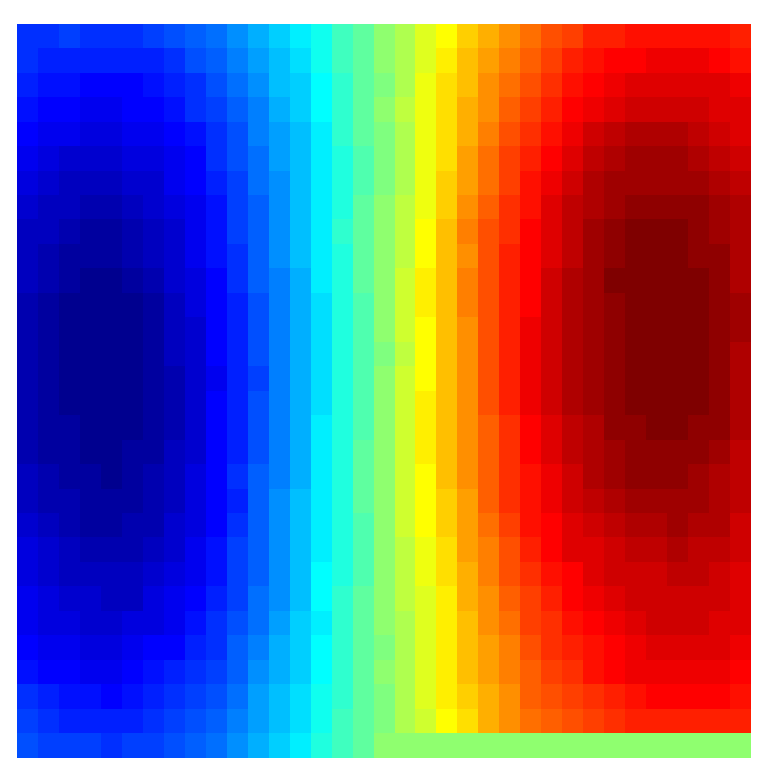
\includegraphics[width=1\textwidth]{Q2a-eig2}}%
\end{minipage}%
\begin{minipage}[t]{0.5\columnwidth}%
\subfloat[Eigenvector 3]{\centering{}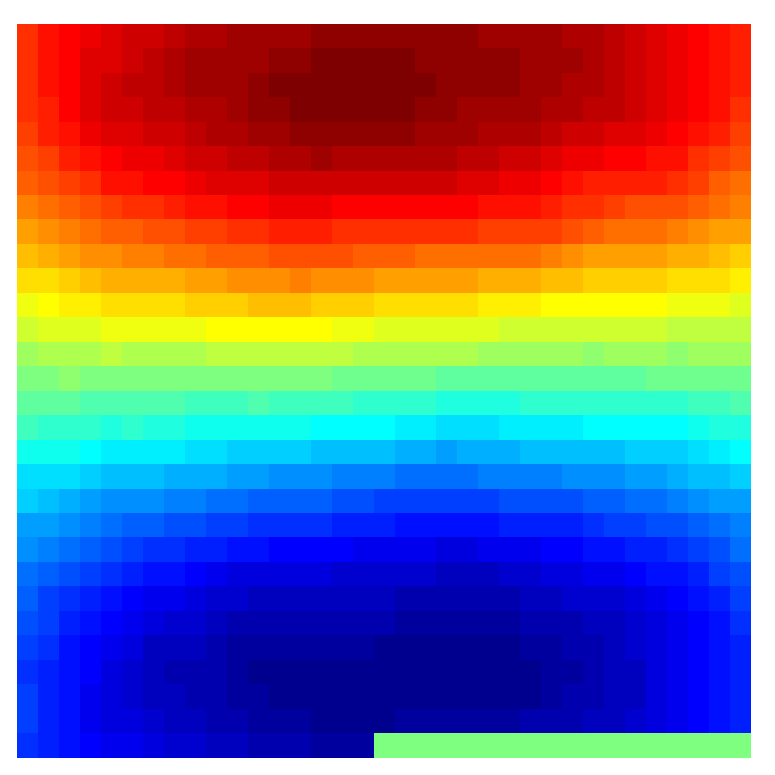
\includegraphics[width=1\textwidth]{Q2a-eig3}}%
\end{minipage}
\par\end{centering}

\caption{Results of PCA Analysis}
\label{fig:q2a}
\end{figure}



\subsection*{b)}

We project all the patches onto the first 3 eigenvectors and then
reconstruct them. We find the patch with the greatest reconstruction
error.

\medskip{}


\lstinputlisting[basicstyle={\scriptsize\ttfamily},breaklines=true,caption={projectSequence.m},captionpos=b,commentstyle={\color{OliveGreen}},frame=tb,language=Matlab]{projectSequence.m}

\medskip{}
\lstinputlisting[basicstyle={\scriptsize\ttfamily},breaklines=true,captionpos=b,commentstyle={\color{OliveGreen}},frame=tb]{q2b.log}

We visualise this patch and its reconstruction in Figure \ref{fig:q2b}.
The pattern of alternating stripes cannot be reproduced from the three
first eigenvectors we saw above.

\begin{figure}[H]
\begin{centering}
\begin{minipage}[t]{0.5\columnwidth}%
\subfloat[Original Patch]{\centering{}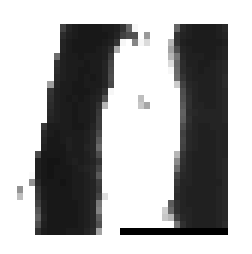
\includegraphics[width=1\textwidth]{Q2b-patch}}%
\end{minipage}%
\begin{minipage}[t]{0.5\columnwidth}%
\subfloat[Reconstruction]{\centering{}
\includegraphics[width=1\textwidth]{Q2b-reconstructed}}%
\end{minipage}
\par\end{centering}

\caption{Patch with worst reconstruction error}
\label{fig:q2b}
\end{figure}



\subsection*{c)}

We visualise the histogram of the target values. This is shown in
Figure \ref{fig:q2c}. It is bimodal with the second mode being very
small. It looks like underlying unimodal with saturation at 63.

\begin{figure}[H]
\begin{centering}
\includegraphics[width=1\textwidth]{Q2c-hist}
\par\end{centering}

\caption{Histogram of Targets}
\label{fig:q2c}

\end{figure}



\subsection*{d)}

We visualise the histogram of differences between x(end) and y --
between the last data pixel and the target pixel. Although the question
specifies 64 bins for the histogram, I later opted to use as many
bins as we had unique values since I found the resulting histogram
clearer. This is shown in Figure \ref{fig:q2d}.

\begin{figure}[H]
\begin{centering}
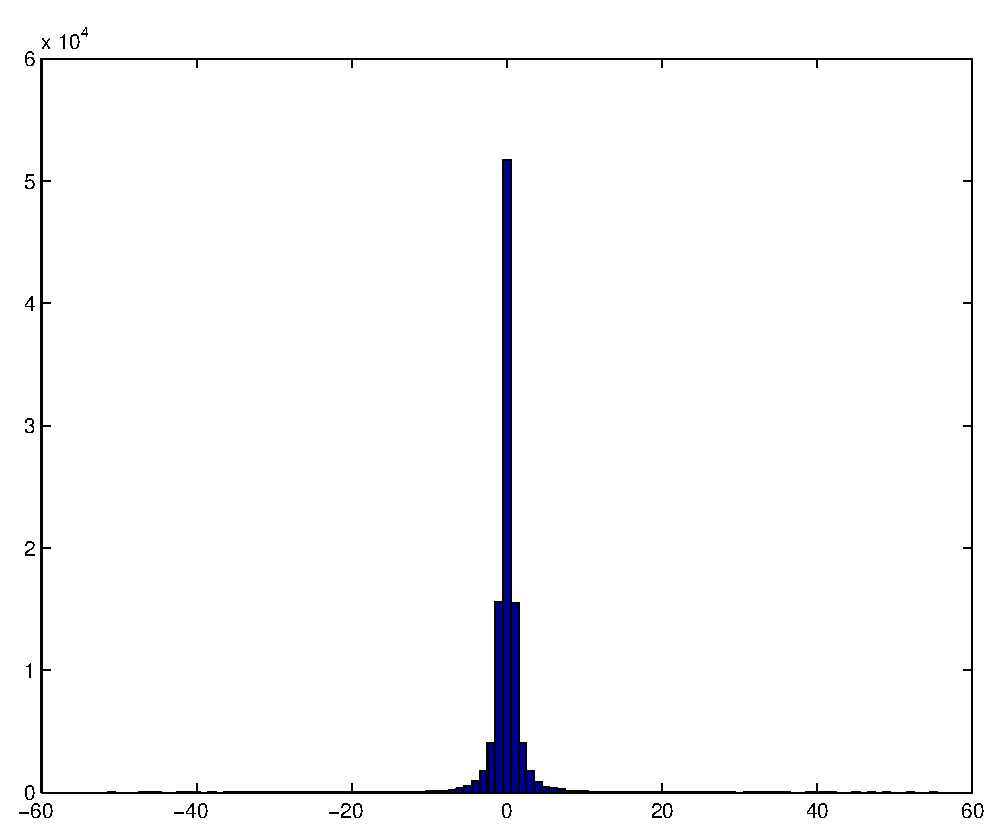
\includegraphics[width=1\textwidth]{Q2d-hist}
\par\end{centering}

\caption{Histogram of Differences}
\label{fig:q2d}
\end{figure}
\medskip{}


\lstinputlisting[basicstyle={\scriptsize\ttfamily},breaklines=true,caption={q2.m},captionpos=b,commentstyle={\color{OliveGreen}},frame=tb,language=Matlab]{q2.m}


\section*{Q3}


\subsection*{a)}

The Maximum Likelihood solution to Naive Bayes with categorical features
and output simply counts instances of each value of $y$ and of $x|y$
in the training set. The main issue with this is that any value of
$y$, or any value of $x$ for a certain $y$, that was not seen in
the training set will be assigned a probability of $0$. One solution
to this is to use additive solution by adding a small increment (for
example, $1$) to each count.


\subsection*{b)}


\subsubsection*{i)}

In the Bayesian formulation of the categorical Naive Bayes model,
we compute $P(Y|X)$ by modelling $P(Y)$ and $P(X|Y)$. Using the
Naive Bayes assumption that the components of $X$ are independent
given the class $Y$, we further break this down into $P(X1|Y)$,
$P(X3|Y)$, $P(X3|Y)$.

We place a conjugate prior over the parameters of our categorical
distributions. The parameters of $P(Y)$ are simply a vector of probabilities
for each value of $Y$; and for each value of $Y$, the parameters
of $P(X_{1}|Y)$ are simply a vector of probabilities for each value
of $X_{1}$; similarly for $X_{2}$ and $X_{3}$.

The conjugate prior for a multinomial distribution is the Dirichlet
distribution, and the categorical distribution is a multinomial distribution
in the case of a single trial. Let $P(Y=y)=\theta_{y}$ be the parameters
of $P(Y)$. Our prior over the parameters $\theta$ is $P(\theta)=Dir(\theta;\alpha)$,
where $\alpha$ are the parameters of the Dirichlet distribution.
We use $\alpha_{k}=1$ to give us a uniform prior over $\theta$.

Since the Dirichlet distribution is a conjugate prior to our $P(Y|\theta)$,
$P(\theta|D)=Dir(\theta;\alpha')$ for some $\alpha'$. Looking this
up on Wikipedia's page on Conjugate Priors we find that $\alpha'_{k}=\alpha_{k}+\sum_{i}I(x^{(i)}=k)$;
in other words, we add to each component of alpha the counts of the
corresponding value in the training data.

We now have a distribution over the parameters of $P(Y|\theta)$,
but we wish to find $P(Y)$ so that we can calculate $P(Y|X)$. To
to this we multiply $P(Y|\theta)$ by $P(\theta)$ and marginalise
out $\theta$ (marginalising out each of its components).

$P(Y=y)=\int_{\{\theta_{i}\}}P(Y=y|\theta)P(\theta)$

$=\int_{\theta_{i}}\theta_{y}Dir(\theta;\alpha)$

We split the integral between the one over \textbackslash{}theta\_y
and the ones over the other components of \textbackslash{}theta.

$=\int_{\theta_{y}}\theta_{y}\int_{\{\theta_{i}\neq y\}}Dir(\theta;\alpha)$

The marginalisation of a Dirichlet distribution is a Beta distribution.

$=\int_{\theta_{y}}\theta_{y}Beta(\theta;\alpha_{y},\alpha_{0}-\alpha_{y})$

Where $\alpha_{0}$ is $\sum_{i}\alpha_{i}$. This expression is now
equivalent to the mean or expectation of our Beta distribution, which
is:

$=\frac{\alpha_{y}}{\alpha_{0}}$

Similar calculations occur for the parameters of $P(X_{k}|Y=y)$ for
each value of Y. We now see that, with a uniform Dirichlet prior with
$\alpha_{k}=1$, the computations and results of the Bayesian formulation
are precisely the same as those of the Maximum Likelihood formulation
with +1 Additive Smoothing.

We train and evaluate the model using 4-fold cross-validation.

\medskip{}


\lstinputlisting[basicstyle={\scriptsize\ttfamily},breaklines=true,caption={crossValidation.m},captionpos=b,commentstyle={\color{OliveGreen}},frame=tb,language=Matlab]{crossValidation.m}

\medskip{}


\lstinputlisting[basicstyle={\scriptsize\ttfamily},breaklines=true,caption={trainAndTestNB.m},captionpos=b,commentstyle={\color{OliveGreen}},frame=tb,language=Matlab]{trainAndTestNB.m}

\medskip{}


\lstinputlisting[basicstyle={\scriptsize\ttfamily},breaklines=true,caption={trainNB.m},captionpos=b,commentstyle={\color{OliveGreen}},frame=tb,language=Matlab]{trainNB.m}

\medskip{}


\lstinputlisting[basicstyle={\scriptsize\ttfamily},breaklines=true,caption={probNB.m},captionpos=b,commentstyle={\color{OliveGreen}},frame=tb,language=Matlab]{probNB.m}

\medskip{}


\lstinputlisting[basicstyle={\scriptsize\ttfamily},breaklines=true,caption={distNB.m},captionpos=b,commentstyle={\color{OliveGreen}},frame=tb,language=Matlab]{distNB.m}

\medskip{}


\lstinputlisting[basicstyle={\scriptsize\ttfamily},breaklines=true,caption={perplexity.m},captionpos=b,commentstyle={\color{OliveGreen}},frame=tb,language=Matlab]{perplexity.m}

We compute the following perplexity value:

\medskip{}
\lstinputlisting[basicstyle={\scriptsize\ttfamily},breaklines=true,captionpos=b,commentstyle={\color{OliveGreen}},frame=tb]{q3bi.log}

This seems like a pretty good value, since the best possible perplexity
score would be 1.


\subsubsection*{ii)}

We visualise $P(y|x^{(i)})$ and $y^{(i)}$ for each fold for (arbitrarily)
the $9465^{th}$ patch in each fold. This is shown in Figure \ref{fig:q3bii}.
The distributions have a sharp peak, and we see that we can get a
mode very close to the true value yet still assign a low probability
to the true value. This is most visible in the example from fold 1.
The disadvantage of our model is that the target values are categorical,
but we know that the underlying reality of the data is a real value
which has been captured with noise and then quantised; if we see an
output value of 45 in the training data it ought to increase our estimated
probability of seeing a 44 or 46, for example.

\begin{figure}[H]
\begin{centering}
\begin{minipage}[t]{0.5\columnwidth}%
\subfloat[Fold 1, Test Patch 9465]{\centering{}\includegraphics[width=1\textwidth]{Q3bii-hist-1-9465}}%
\end{minipage}%
\begin{minipage}[t]{0.5\columnwidth}%
\subfloat[Fold 2, Test Patch 9465]{\centering{}\includegraphics[width=1\textwidth]{Q3bii-hist-2-9465}}%
\end{minipage}
\par\end{centering}

\begin{centering}
\begin{minipage}[t]{0.5\columnwidth}%
\subfloat[Fold 3, Test Patch 9465]{\centering{}\includegraphics[width=1\textwidth]{Q3bii-hist-3-9465}}%
\end{minipage}%
\begin{minipage}[t]{0.5\columnwidth}%
\subfloat[Fold 4, Test Patch 9465]{\centering{}\includegraphics[width=1\textwidth]{Q3bii-hist-4-9465}}%
\end{minipage}
\par\end{centering}

\caption{Distributions and actual values for selected test patches}
\label{fig:q3bii}
\end{figure}



\subsubsection*{iii)}

The strong assumption made by Naive Bayes is that the input features
are distributed independently given the output value. This seems unlikely,
especially since we could have picked any other pixel in the patch
as the target; and if the Naive Bayes assumption held for one target
then it seems like it should equally hold for another, since there
is little to distinguish them; but it would therefore have to hold
between any sets of pixels in the patch.

\medskip{}


\lstinputlisting[basicstyle={\scriptsize\ttfamily},breaklines=true,caption={q3.m},captionpos=b,commentstyle={\color{OliveGreen}},frame=tb,language=Matlab]{q3.m}


\section*{Q4}

I interpret this question as asking us to now treat the intput and
output as numerical rather than categorical data and perform linear
regression on that.


\subsection*{a)}

We use Netlab to perform linear regression, although this is more
to save time debugging than due to any particular difficulty of implementation.
We select only the final, 34th and 35th from final pixels in the patch
data for our input, as specified.

\medskip{}


\lstinputlisting[basicstyle={\scriptsize\ttfamily},breaklines=true,caption={trainAndTestLR.m},captionpos=b,commentstyle={\color{OliveGreen}},frame=tb,language=Matlab]{trainAndTestLR.m}

\medskip{}


\lstinputlisting[basicstyle={\scriptsize\ttfamily},breaklines=true,caption={trainLR.m},captionpos=b,commentstyle={\color{OliveGreen}},frame=tb,language=Matlab]{trainLR.m}

\medskip{}


\lstinputlisting[basicstyle={\scriptsize\ttfamily},breaklines=true,caption={probLR.m},captionpos=b,commentstyle={\color{OliveGreen}},frame=tb,language=Matlab]{probLR.m}

We measure the perplexity under cross-validation.

\medskip{}
\lstinputlisting[basicstyle={\scriptsize\ttfamily},breaklines=true,captionpos=b,commentstyle={\color{OliveGreen}},frame=tb]{q4a.log}

It might seem wrong to compare this to the perplexity in the last
section, since here $p(y|x)$ is a probability density rather than
a discrete probability. Perhaps it would have been better to approximate
$P(y|x)$ as $1/2*(p(y-0.5|x)+p(y+0.5|x))$, thus approximating the
integral of $p(y|x)$ in the interval $(y-0.5,\; y+0.5)$. But numerically
this would give very similar results to just our evaluation at the
midpoint, so we do allow ourselves to compare the results using a
$p(y|x)$ as a density function to those using $P(y|x)$.


\subsection*{b)}

We project the data onto the first ten eigenvectors of our PCA model
from Q2, and use these as our features for linear regression.

\medskip{}
\lstinputlisting[basicstyle={\scriptsize\ttfamily},breaklines=true,captionpos=b,commentstyle={\color{OliveGreen}},frame=tb]{q4b.log}


\subsection*{c)}

The perplexity score for the PCA method is notably worse. Although
the PCA construction gives us a good way of discarding data while
still reconstructing a reasonable approximation of the original patches
to human eyes, when it comes to predicting specifically the value
of the target pixel, using its neighbours seems better.


\section*{Q5}

The results of Q2d) suggest we could get a decent result by just predicting
y=x(end). We find the standard deviation of the error to give us a
narrow gaussian around x(end) for a distribution p(y|x).

\medskip{}


\lstinputlisting[basicstyle={\scriptsize\ttfamily},breaklines=true,caption={q5.m},captionpos=b,commentstyle={\color{OliveGreen}},frame=tb,language=Matlab]{q5.m}

\medskip{}
\lstinputlisting[basicstyle={\scriptsize\ttfamily},breaklines=true,captionpos=b,commentstyle={\color{OliveGreen}},frame=tb]{q5.log}

The resulting perplexity is comparable to our predictors from Q4 but
not as good as the naive bayes result from Q3.

\medskip{}


\lstinputlisting[basicstyle={\scriptsize\ttfamily},breaklines=true,caption={q4.m},captionpos=b,commentstyle={\color{OliveGreen}},frame=tb,language=Matlab]{q4.m}


\section*{Appendix A - Additional Code}

\medskip{}


\lstinputlisting[basicstyle={\scriptsize\ttfamily},breaklines=true,caption={main.m},captionpos=b,commentstyle={\color{OliveGreen}},frame=tb,language=Matlab]{main.m}

\medskip{}


\lstinputlisting[basicstyle={\scriptsize\ttfamily},breaklines=true,caption={figurePatch.m},captionpos=b,commentstyle={\color{OliveGreen}},frame=tb,language=Matlab]{figurePatch.m}

\medskip{}


\lstinputlisting[basicstyle={\scriptsize\ttfamily},breaklines=true,caption={figureEig.m},captionpos=b,commentstyle={\color{OliveGreen}},frame=tb,language=Matlab]{figureEig.m}

\medskip{}
\lstinputlisting[basicstyle={\scriptsize\ttfamily},breaklines=true,caption={makeLogFile.m},captionpos=b,commentstyle={\color{OliveGreen}},frame=tb,language=Matlab]{makeLogFile.m}

\medskip{}


\lstinputlisting[basicstyle={\scriptsize\ttfamily},breaklines=true,caption={writeFigureEPS.m},captionpos=b,commentstyle={\color{OliveGreen}},frame=tb,language=Matlab]{writeFigureEPS.m}
\end{document}
